\documentclass[../main.tex]{subfiles}
\begin{document}
\chapter{Multivariate Functions: Applications}
\section{Directional Derivatives and Gradient}
Consider $f(x, y)$ and a vector displacement $\d{\vec{s}}=(\d{x}, \d{y})$.
The infinitesimal change in $f$ along $\d{\vec{s}}$ is:
\begin{align*}
  \d{f} &= \pderiv{f}{x}\d{x} + \pderiv{f}{y}\d{y} \\
        &= (\d{x}, \d{y}) \cdot \left(\pderiv{f}{x}, \pderiv{f}{y}\right) \\
        &= \d{\vec{s}} \cdot \nabla f
\end{align*}
where $\nabla f$ is defined as follows.
\begin{definition}[Gradient of $f$]
  The  \textit{gradient of $f$} or grad $f$ is defined to be:
  \[
    \nabla f = \left(\pderiv{f}{x}, \pderiv{f}{y}\right)
  \]
\end{definition}
If we write $\d{\vec{s}} = \d{s}\uvec{s}$, where $\uvec{s}$ is a unit vector, then:
\[
  \d{f} = \d{s}\uvec{s} \cdot \nabla f
\]
\begin{definition}[Directional Derivative]
  The \textit{directional derivative} of $f$ in the direction of $\uvec{s}$ is:
  \[
    \deriv{f}{s} = \uvec{s} \cdot \nabla f
  \]
  where $\uvec{s}$ is a unit vector.
  This tells us the rate of change of $f(x, y)$ in the direction of $\uvec{s}$.
\end{definition}
\begin{center}
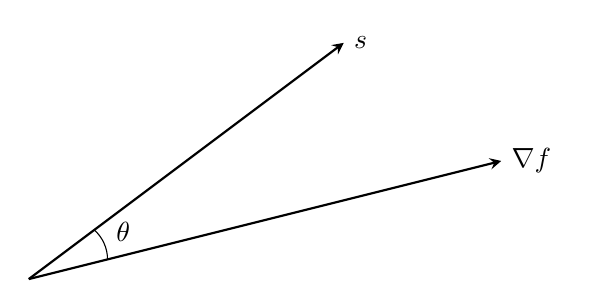
\begin{tikzpicture}[>=stealth, scale=1]
  \draw[->, thick] (0, 0) -- (4, 3) node[right] {$\uvec{s}$};
  \draw[->, thick] (0, 0) -- (6, 1.5) node[right] {$\nabla f$};

  \draw (1,0.25) arc[start angle=0, end angle=49, radius=0.5];

  \node at (1.2,0.6) {$\theta$};
\end{tikzpicture}
\end{center}
Using the definition of the scalar product, we see that:
\[
  \deriv{f}{s} = \uvec{s} \cdot \nabla f = \cos \theta |\nabla f|
\]
\begin{remark}[Note]
  As an alternative, we could have defined $\nabla f$ geometrically as the vector such that:
  \[
    \deriv{f}{s} = \uvec{s} \cdot \nabla f
  \]
  for all $\uvec{s}$.
\end{remark}
\subsection{Properties of the Gradient Vector}
\begin{enumerate}
  \item Direction of $\nabla f$ is that in which $f$ \textbf{increases} most rapidly as the directional derivative is greatest when $\uvec{s}$ is parallel to $\nabla f$
  \item The magnitude of $\nabla f$ is the max rate of change of $f$ at a particular point:
    \[
      |\nabla f| = \max_{\forall \theta}\left(\deriv{f}{s}\right)
    \]
  \item If $\uvec{s}$ is parallel to contours of $f$ (curves of constant $f$), then:
    \[
      \deriv{f}{s} = 0 = \uvec{s} \cdot \nabla f
    \]
    Therefore, $\nabla f$ is perpendicular to the contours of $f$.
\end{enumerate}
\section{Stationary Points}
There is always at least one direction where $\deriv{f}{s} = 0$, i.e. when $\uvec{s}$ is parallel to the contours of $f$.
So to define the notion of a stationary point, we require that $\deriv{f}{s} = 0$ in all directions, not just that $\deriv{f}{s} = 0$ for some $\uvec{s}$.
\begin{definition}[Stationary Point]
  A stationary point is a point where:
  \[
    \deriv{f}{s} = 0\ \forall \uvec{s}
  \]
\end{definition}
So at stationary points:
\[
  \vec{s} \cdot \nabla f = 0\ \forall \uvec{s} \implies \nabla f = \vec{0}
\]
\subsection{Types of Stationary Points}
\label{typesOfStationary}
\subsubsection{Local Maximum}
For a local maximum, $\nabla f$ points towards the maximum point.
Contours are usually locally elliptical around a maximum.
\begin{center}
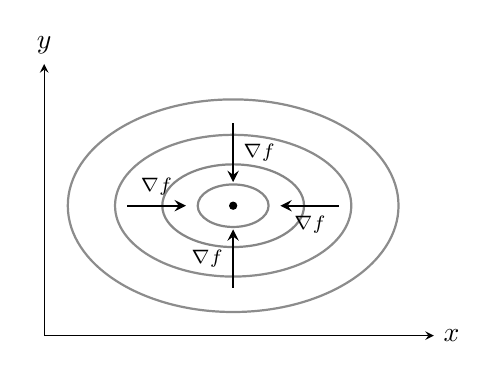
\begin{tikzpicture}[>=stealth, scale=1.5]
\draw[->] (0,0) -- (3.3,0) node[right] {$x$};
\draw[->] (0,0) -- (0,2.3) node[above] {$y$};

\def\cx{1.6}
\def\cy{1.1}

\draw[thick, gray!95] (\cx,\cy) ellipse (0.3 and 0.18);
\draw[thick, gray!95] (\cx,\cy) ellipse (0.6 and 0.35);
\draw[thick, gray!90] (\cx,\cy) ellipse (1.0 and 0.6);
\draw[thick, gray!90] (\cx,\cy) ellipse (1.4 and 0.9);

\fill (\cx,\cy) circle (1pt);

\draw[<-, thick] (\cx,\cy) + (0, -0.2) -- +(0, -0.7) node[midway, left] {$\scriptstyle\nabla f$};
\draw[<-, thick] (\cx,\cy) + (0, 0.2) -- +(0, 0.7) node[midway, right] {$\scriptstyle\nabla f$};
\draw[<-, thick] (\cx,\cy) + (0.4, 0) -- +(0.9, 0) node[midway, below] {$\scriptstyle\nabla f$};
\draw[<-, thick] (\cx,\cy) + (-0.4, 0) -- +(-0.9, 0) node[midway, above] {$\scriptstyle\nabla f$};
\end{tikzpicture}
\end{center}
\subsubsection{Local Minimum}
For a local minimum, $\nabla f$ points away from the minimum point.
Again, contours are usually locally elliptical.
\begin{center}
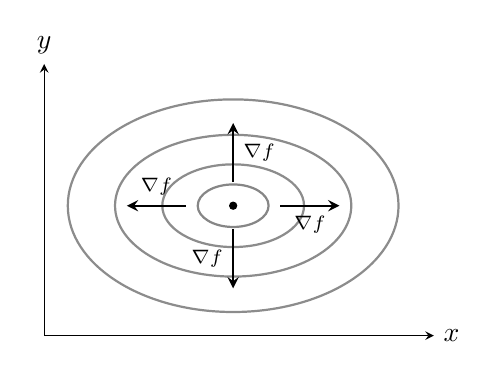
\begin{tikzpicture}[>=stealth, scale=1.5]
\draw[->] (0,0) -- (3.3,0) node[right] {$x$};
\draw[->] (0,0) -- (0,2.3) node[above] {$y$};

\def\cx{1.6}
\def\cy{1.1}

\draw[thick, gray!95] (\cx,\cy) ellipse (0.3 and 0.18);
\draw[thick, gray!90] (\cx,\cy) ellipse (0.6 and 0.35);
\draw[thick, gray!90] (\cx,\cy) ellipse (1.0 and 0.6);
\draw[thick, gray!90] (\cx,\cy) ellipse (1.4 and 0.9);

\fill (\cx,\cy) circle (1pt);

\draw[->, thick] (\cx,\cy) + (0, -0.2) -- +(0, -0.7) node[midway, left] {$\scriptstyle\nabla f$};
\draw[->, thick] (\cx,\cy) + (0, 0.2) -- +(0, 0.7) node[midway, right] {$\scriptstyle\nabla f$};
\draw[->, thick] (\cx,\cy) + (0.4, 0) -- +(0.9, 0) node[midway, below] {$\scriptstyle\nabla f$};
\draw[->, thick] (\cx,\cy) + (-0.4, 0) -- +(-0.9, 0) node[midway, above] {$\scriptstyle\nabla f$};
\end{tikzpicture}
\end{center}
\subsubsection{Saddle Point}
A saddle point is \textbf{not} a local extremum.
Generally speaking, in one direction it is a maximum and in another direction it is a minimum.
Contours always cross and only ever cross at a saddle points.
Around a saddle point, the contours are usually locally hyperbolic.
\begin{center}
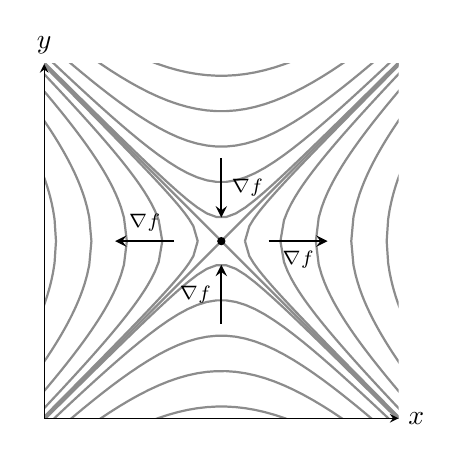
\begin{tikzpicture}[scale=1.5, >=stealth]
\def\cx{1.5}
\def\cy{1.5}
\begin{scope}
\clip (0, 0) rectangle (3, 3);
\foreach \b in {0.2, 0.5, 0.8, 1.1, 1.4}{
    \draw[thick, gray!90, domain=\cx+\b:\cx+2, samples=50] plot ({\x}, {\cy + sqrt((\x-\cx)^2 - \b^2)});
    \draw[thick, gray!90, domain=\cx+\b:\cx+2, samples=50] plot ({\x}, {\cy - sqrt((\x-\cx)^2 - \b^2)});
    \begin{scope}[xscale=-1, xshift=-3cm]
      \draw[thick, gray!90, domain=\cx+\b:\cx+2, samples=50] plot ({\x}, {\cy + sqrt((\x-\cx)^2 - \b^2)});
      \draw[thick, gray!90, domain=\cx+\b:\cx+2, samples=50] plot ({\x}, {\cy - sqrt((\x-\cx)^2 - \b^2)});
    \end{scope}
    \draw[thick, gray!90, domain=\cx-2:\cx+2, samples=50] plot ({\x}, {\cy + sqrt((\x-\cx)^2 + \b^2)});
    \draw[thick, gray!90, domain=\cx-2:\cx+2, samples=50] plot ({\x}, {\cy - sqrt((\x-\cx)^2 + \b^2)});
}
\draw[thick, gray!90] (\cx, \cy) + (-2, -2) -- +(2, 2);
\draw[thick, gray!90] (\cx, \cy) + (2, -2) -- +(-2, 2);
\end{scope}

\fill (\cx,\cy) circle (1pt);
\draw[<-, thick] (\cx,\cy) + (0, -0.2) -- +(0, -0.7) node[midway, left] {$\scriptstyle\nabla f$};
\draw[<-, thick] (\cx,\cy) + (0, 0.2) -- +(0, 0.7) node[midway, right] {$\scriptstyle\nabla f$};
\draw[->, thick] (\cx,\cy) + (0.4, 0) -- +(0.9, 0) node[midway, below] {$\scriptstyle\nabla f$};
\draw[->, thick] (\cx,\cy) + (-0.4, 0) -- +(-0.9, 0) node[midway, above] {$\scriptstyle\nabla f$};

\draw[->] (0,0) -- (3,0) node[right] {$x$};
\draw[->] (0,0) -- (0,3) node[above] {$y$};
\end{tikzpicture}
\end{center}
\section{Classification of Stationary Points}
How does $f$ change in the vicinity of a stationary point?
\subsection{Taylor Series for Multivariate Functions}
Consider how $f(x, y)$ varies along the line $\vec{x}(s) = \vec{x}_0 + s \uvec{s}$.
\begin{center}
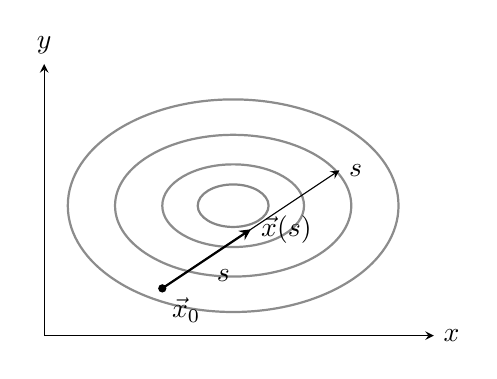
\begin{tikzpicture}[>=stealth, scale=1.5]
\draw[->] (0,0) -- (3.3,0) node[right] {$x$};
\draw[->] (0,0) -- (0,2.3) node[above] {$y$};

\def\cx{1.6}
\def\cy{1.1}

\draw[thick, gray!95] (\cx,\cy) ellipse (0.3 and 0.18);
\draw[thick, gray!90] (\cx,\cy) ellipse (0.6 and 0.35);
\draw[thick, gray!90] (\cx,\cy) ellipse (1.0 and 0.6);
\draw[thick, gray!90] (\cx,\cy) ellipse (1.4 and 0.9);

\coordinate (X) at (1, 0.4);
\fill (X) circle (1pt) node[below right] {$\vec{x}_0$};
\draw[->] (X) -- +(1.5, 1) node[right] {$\uvec{s}$};
\draw[->, thick] (X) -- +(0.75, 0.5) node[right] {$\vec{x}(s)$} node[midway, below right] {$s$};
\end{tikzpicture}
\end{center}
Along this line, $f(\vec{x}_0 + s \uvec{s}) = f(x(s), y(s))$ so $f$ is a function of $s$.
Therefore, we can use the usual Taylor series:
\begin{align*}
  f(\vec{x}_0 + s \uvec{s}) &= f(\vec{x}_0) + s \at{\deriv{f}{s}}{\vec{x}_0} + \frac{1}{2}s^2 \at{\deriv[2]{f}{s}}{\vec{x}_0} + \cdots \\
                            &= f(\vec{x}_0) + s \uvec{s} \cdot \at{\nabla f}{\vec{x}_0} + \frac{1}{2}s^2 \at{(\uvec{s} \cdot \nabla)(\uvec{s} \cdot \nabla f)}{\vec{x}_0} + \cdots
\end{align*}
Looking at the second term of the expansion, let $\delta\vec{x} = (x - x_0, y - y_0) = (\delta x, \delta y) = s \uvec{s}$.
We then have:
\[
  s \uvec{s} \cdot \nabla f = \delta \vec{x} \cdot \nabla f = \delta x \pderiv{f}{x} + \delta y \pderiv{f}{y}
\]
Looking at the third term of the expansion, let $\hat{s}_x$ and $\hat{s}_y$ be the components of $\uvec{s} =(\hat{s}_x, \hat{s}_y)$.
We then have:
\begin{align*}
  s^2(\uvec{s} \cdot \nabla)(\uvec{s} \cdot \nabla f) &= s^2\left(\hat{s}_x \pderiv{}{x} + \hat{s}_y \pderiv{}{y}\right)\left(\hat{s}_x \pderiv{f}{x} + \hat{s}_y \pderiv{f}{y}\right) \\
                                                      &= \left(\delta x \pderiv{}{x} + \delta y \pderiv{}{y}\right)\left(\delta x \pderiv{f}{x} + \delta y \pderiv{f}{y}\right) \\
                                                      &= (\delta x)^2 \pderiv[2]{f}{x} + (\delta x)(\delta y) \frac{\partial^2 f}{\partial x \partial y} + (\delta y)(\delta x)\frac{\partial^2 f}{\partial y \partial x} + (\delta y)^2 \pderiv[2]{f}{y} \\
                                                      &= (\delta x, \delta y)
                                                      \begin{pmatrix}
                                                      f_{x x} & f_{x y} \\
                                                      f_{y x} & f_{y y} \\
                                                      \end{pmatrix}
                                                      \begin{pmatrix}
                                                      \delta x \\
                                                      \delta y \\
                                                      \end{pmatrix}
\end{align*}
\begin{definition}[Hessian Matrix]
  The \textit{Hessian Matrix} is defined to be:
  \[
    H = \nabla \nabla f = \begin{pmatrix}
    f_{x x} & f_{x y} \\
    f_{y x} & f_{y y} \\
    \end{pmatrix}
  \]
  This is symmetric as $f_{x y} = f_{y x}$.
\end{definition}
The multivariate Taylor series is then:
\begin{align*}
  f(x_0 + \delta x, y_0 + \delta y) &= f(x_0, y_0) + \at{\left[\delta x \pderiv{f}{x} + \delta y \pderiv{f}{y}\right]}{(x_0, y_0)} \\ &\quad+\frac{1}{2}\at{\left[(\delta x)^2 \pderiv[2]{f}{x} + 2\delta x\delta y \frac{\partial^2 f}{\partial x \partial y} + (\delta y)^2 \pderiv[2]{f}{y}\right]}{(x_0, y_0)} + \cdots
\end{align*}
This can be written in a coordinate independent form as:
\begin{align*}
  f(\vec{x}_0 + \delta \vec{x}) &= f(\vec{x}_0) + \delta \vec{x} \cdot \at{(\nabla f)}{\vec{x}_0} + \frac{1}{2} (\delta \vec{x})^{\trans} \at{H}{\vec{x}_0} \delta \vec{x} + \cdots \\
                                & =f(\vec{x}_0) + \delta \vec{x} \cdot \at{(\nabla f)}{\vec{x}_0} + \frac{1}{2} (\delta \vec{x})^{\trans} \at{(\nabla \nabla f)}{\vec{x}_0} \delta \vec{x} + \cdots
\end{align*}
\subsection{Classification of Stationary Points}
Suppose $\vec{x}_0$ is a stationary point, that is $\at{\nabla f}{\vec{x}_0} = \vec{0}$.

Using the multivariate Taylor series, around $\vec{x}_0$ we have:
\[
  f(\vec{x}) \approx f(\vec{x}_0) + \frac{1}{2} (\delta \vec{x})^{\trans} H (\delta\vec{x})
\]
where $\delta \vec{x} = \vec{x} - \vec{x}_0$.
\begin{definition}[Positive and Negative Definite]
  A real symmetric matrix $H$ is:
  \begin{itemize}
    \item \textit{Positive definite}, if:
      \[
        \vec{x}^{\trans} H \vec{x} > 0\ \forall \vec{x} \in \R^{n}, \vec{x} \neq \vec{0}
      \]
    \item \textit{Negative definite}, if:
      \[
        \vec{x}^{\trans} H \vec{x} < 0\ \forall \vec{x} \in \R^{n}, \vec{x} \neq \vec{0}
      \]
    \item \textit{Indefinite} otherwise.
  \end{itemize}
\end{definition}
\begin{itemize}
  \item If $H$ is \textbf{positive definite} at $\vec{x}_0$, then the stationary point is a local minimum as $f(\vec{x}) > f(\vec{x}_0)$ close to $\vec{x}_0$.
  \item If $H$ is \textbf{negative definite} at $\vec{x}_0$, then the stationary point is a local maximum as $f(\vec{x}) < f(\vec{x}_0)$ close to $\vec{x}_0$.
  \item If $H$ is \textbf{indefinite}, then the stationary point may be a maximum, minimum or a saddle point.
\end{itemize}
\subsection{Definiteness and Eigenvalues}
$H$ is a real symmetric matrix, therefore it can be diagonalised with an orthogonal transformation. This corresponds to using coordinates along the principal axes (that is, the axes defined by the eigenvectors).
\textit{(For more details see Vectors and Matrices 4.6)}

After diagonalisation, in $n$ dimensions:
\begin{align*}
  (\delta \vec{x})^{\trans}H(\delta\vec{x}) &= (\delta x_1, \ldots, \delta x_n)
  \begin{pmatrix}
  \lambda_1 &  &  \\
   & \ddots &  \\
   &  & \lambda_n \\
  \end{pmatrix}
  \begin{pmatrix}
  \delta x_1 \\
  \vdots \\
  \delta x_n \\
  \end{pmatrix} \\
  &= \lambda_1 (\delta x_1)^2 + \lambda_2 (\delta x_2)^2 + \cdots + \lambda_n(\delta x_n)^2
\end{align*}
where $\delta x_i$ are the coordinates with respect to the principal axes.

Since the definiteness of $H$ depends on whether the relation holds for all $\delta \vec{x}$, we can conclude that:
\begin{itemize}
  \item $H$ is \textbf{positive definite} if and only if all $\lambda_i > 0$ $\to$ \textbf{Minimum} point.
  \item $H$ is \textbf{negative definite} if and only if all $\lambda_i < 0$ $\to$ \textbf{Maximum} point.
  \item All eigenvalues are \textbf{non-zero and mixed signs} $\to$ \textbf{Saddle} point.
  \item \textbf{Any} eigenvalues are 0 $\to$ Need higher order terms in the Taylor series to classify the stationary point.
\end{itemize}
\begin{example}
  \[
    f(x, y) = x^2 + y^4
  \]
  We can see that is has a global minimum at $(0, 0)$.
  First we find $\nabla f$:
  \[
    \nabla f = (f_x, f_y) = (2x, 4y^3)
  \]
  We then can find the Hessian at $(0, 0)$:
  \[
    H = \begin{pmatrix}
    2 & 0 \\
    0 & 12y^2 \\
    \end{pmatrix} \implies
    \at{H}{(0, 0)} =
    \begin{pmatrix}
    2 & 0 \\
    0 & 0 \\
    \end{pmatrix}
  \]
  which has eigenvalues $\lambda_1 = 2$ and $\lambda_2 = 0$.
  Since one of the eigenvalues is 0, we would need to use higher order terms in the Taylor series to classify the stationary point using this method.
\end{example}
\subsection{Definiteness and Signature}
The signature of the Hessian matrix provides an alternative method for classifying stationary points that does not involve computing eigenvalues.

\begin{definition}[Signature]
  The \textit{signature} of $H$ is the pattern of signs of the ordered sub-determinants of the leading principal minors of $H$.
\end{definition}
For $f(x_1, x_2, \ldots, x_n)$, the sub-determinants of the leading principal minors of $H$ are:
\begin{align*}
  |H_1| &= |f_{x_1 x_1}| \\
  |H_2| &= \begin{vmatrix}
  f_{x_1 x_1} & f_{x_1 x_2} \\
  f_{x_2 x_1} & f_{x_2 x_2} \\
  \end{vmatrix} \\
  &\ \ \vdots \\
  |H_n| &= \begin{vmatrix}
  f_{x_1 x_1} & \cdots & f_{x_1 x_n} \\
  \vdots & \ddots & \vdots \\
  f_{x_n x_1} & \cdots & f_{x_nx_n } \\
  \end{vmatrix}
\end{align*}
So the signature of $H$ is: sign of $|H_1|$, sign of $|H_2|$, ..., sign of $|H_n|$.
\begin{theorem}[Slyvesters Critereon]
  \label{syvestersCritereon}
  For a symmetric matrix $H$:
  \begin{align*}
    H \text{ is positive definite} &\iff \text{ signature is: }+, +, +, \cdots, +\\
    H \text{ is negative definite} &\iff \text{ signature is: }-, +, -, +, \cdots
  \end{align*}
  If $H$ has any other signature, it is indefinite.
\end{theorem}
\subsection{Contours Near Stationary Points}
Suppose $f(x, y)$ has a stationary point at $\vec{x}_0 = (x_0, y_0)$.
For ease, use the coordinates aligned with the principal axes of $H(\vec{x}_0)$.
So $H(\vec{x}_0)$ will be diagonal:
\[
  H(\vec{x}_0) = \begin{pmatrix}
  \lambda_1 & 0 \\
  0 & \lambda_2 \\
  \end{pmatrix}
\]
We are going to assume the eigenvalues are non-zero for simplicity.
Consider $\delta \vec{x} = (\xi, \eta)$ for small $\xi$ and $\eta$.
\[
  \vec{x} = \vec{x}_0 + (\xi, \eta)
\]
Then around $\vec{x}_0$ we  have:
\[
  f(\vec{x}) = f(\vec{x}_0) + \frac{1}{2}(\lambda_1 \xi^2 + \lambda_2 \eta^2) + \cdots
\]
Close to $\vec{x}_0$, the higher order terms become negligible.
Therefore, close to $\vec{x}_0$ the contours have the form:
\[
  \lambda_1 \xi^2 + \lambda_2 \eta^2 = \text{constant}
\]
For a maximum or minimum, both eigenvalues share the same sign so we see that this describes an ellipse with respect to the principal axes of $H(\vec{x}_0)$.

At  a saddle point, the eigenvalues have opposite signs so we see that describes a hyperbola with respect to the principal axes of $H(\vec{x}_0)$.

This agrees with what we saw in \cref{typesOfStationary}.
\subsection{Example of Classifying Stationary Points}
\begin{example}
  Find and classify the stationary points of:
  \[
    f(x, y) = 4x^3 - 12xy + y^2 + 10y+ 6
  \]
  \begin{align*}
    \nabla f = (f_x, f_y) = (12x^2 - 12y, -12x + 2y + 10)
  \end{align*}
  We have stationary points when both $f_x$ and $f_y$ are 0.
  \begin{align*}
    f_x &= 0 \implies y = x^2 \\
    f_y &= 0 \implies -12x + 2y + 10 = 0
  \end{align*}
  Combining the above we have:
  \begin{align*}
    -12x + 2x^2 + 10 &= 0 \\
    x^2 - 6x + 5 &= 0
  \end{align*}
  This has roots at $x = 1$ and $x = 5$.
  Therefore the stationary points are at $(1, 1)$ and $(5, 25)$.

  Now to compute the Hessian we first find:
  \[
    f_{x x} = 24x,\ f_{x y} = -12,\ f_{y y} = 2
  \]
  So:
  \[
    H = \begin{pmatrix}
    24x & -12 \\
    -12 & 2 \\
    \end{pmatrix}
  \]
  First, considering the stationary point $(1, 1)$:
  \[
    \at{H}{(1, 1)} = \begin{pmatrix}
    24 & -12 \\
    -12 & 2 \\
    \end{pmatrix}
  \]
  So $|H_1| = 24$ and $|H_2| = -96$.
  So the signature is $+, -$ which doesn't match either of the conditions in \cref{syvestersCritereon}, thus $H$ is indefinite.
  Since the diagonalised form of $H$ has the same determinant and $|H| \neq 0$, the product of all eigenvalues is non-zero.
  Therefore, all eigenvalues are non-zero and have mixed signs so we have a saddle point.

  Now, considering the stationary point $(5, 25)$
  \[
    \at{H}{(5, 25)} = \begin{pmatrix}
    120 & -12 \\
    -12 & 2 \\
    \end{pmatrix}
  \]
  So $|H_1| = 120$ and $|H_2| = 240 - 144 = 96$.
  So the signature is $+, +$, so we see from \cref{syvestersCritereon} that $H$ is positive definite.
  Therefore we have a local minimum.

  Near the saddle point, the contours satisfy
  \[
    24(\delta x)^2 - 24(\delta x)(\delta y) + 2(\delta y)^2 = \text{constant}
  \]
  If we find the eigenvalues and eigenvectors of $\at{H}{(5, 25)}$, this will define an ellipse aligned with the principal axes of $\at{H}{(5, 25)}$.

\textit{(For more details see Vectors and Matrices 4.6)}
\end{example}
\section{Systems of Linear ODEs}
Consider $y_1(t)$ and $y_2(t)$ with:
\begin{align*}
  \dot{y}_1 &= ay_1 + by_2 + f_1(t) \\
  \dot{y}_2 &= cy_1 + dy_2 + f_2(t)
\end{align*}
where $a, b, c, d$ are constants.

We can also write this in vector form:
\[
  \dot{\vec{Y}} = M\vec{Y} + \vec{F}
\]
where
\[
  M = \begin{pmatrix}
  a & b \\
  c & d \\
  \end{pmatrix},\
  \vec{Y} = \begin{pmatrix}
  y_1(t) \\
  y_2(t) \\
  \end{pmatrix},\
  F = \begin{pmatrix}
  f_1(t) \\
  f_2(t) \\
  \end{pmatrix}
\]
There are two ways to solve systems like these.
\subsubsection{Convert to higher order ODE for one variable}
We can convert the system into a higher order ODE for a single variable:
\begin{align*}
  \ddot{y}_1 &= a\dot{y}_1 + b\dot{y}_2 + \dot{f}_1 \\
             &= a\dot{y}_1 + b(cy_1 + dy_2 + f_2) + \dot{f}_1  \\
             &= a\dot{y}_1 + bcy_1 + d(\dot{y}_1 - ay_1 - f_1) + bf_2 + \dot{f}_1
\end{align*}
Therefore:
\[
  \ddot{y}_1 - (a + d)\dot{y}_1 + (ad - bc)y_1 = bf_2 - df_1 + \dot{f}_1
\]
So we have a linear second order ODE with constant coefficients.
\subsubsection{Solve directly with matrix methods}
Solving using matrix methods may be more convenient, especially as we generalise to higher order systems.

\begin{remark}
  We may sometimes write a higher order ODE as a set of 1st order ODEs as it can make them more convenient to solve numerically using a computer.

  For example, consider the ODE:
  \[
    \ddot{y} + a\dot{y} + b\dot{y} = f
  \]
  Let $y_1 = y$ and $y_2 = \dot{y}$ so:
  \[
    \dot{y}_1 = y_2,\ \dot{y}_2 = \ddot{y} = -ay_2 -by_1 + f
  \]
  In matrix form this can be written as:
  \[
    \dot{\vec{Y}} = \begin{pmatrix}
    0 & 1 \\
    -b & -a \\
    \end{pmatrix} \vec{Y} +
    \begin{pmatrix}
    0 \\
    f \\
    \end{pmatrix}
  \]
  where $\vec{Y} = \begin{pmatrix}
    y_1 \\
    y_2 \\
    \end{pmatrix}$.
\end{remark}
\subsection{Matrix Methods}
Consider the system:
\[
  \dot{\vec{Y}} = M \vec{Y} + \vec{F}(t)
\]
The process of solving this using matrix methods is quite similar to how we solved 2nd order linear ODEs with constant coefficients in \cref{constantCoeffMethod}.
\begin{enumerate}
\item
  We first write:
  \[
    \vec{Y} = \vec{Y}_c + \vec{Y}_p
  \]
  Where $\vec{Y}_c$ is the complementary function and satisfies the homogeneous equation:
  \[
    \dot{\vec{Y}}_c = M\vec{Y}_c
  \]
  and $\vec{Y}_p$ is the particular integral that satisfies the whole system.
\item
  We then look for $\vec{Y}_c$ of the form:
  \[
    \vec{Y}_c = \vec{v}e^{\lambda t}
  \]
  where $\vec{v}$ is a constant vector.
  \[
    \dot{\vec{Y}}_c = \lambda \vec{v}e^{\lambda t} = \lambda \vec{Y}_c = M\vec{Y}_c \implies e^{\lambda t}(M\vec{v}) = e^{\lambda t}(\lambda \vec{v})
  \]
  Since this is true for all $t$, we must have:
  \[
    M \vec{v} = \lambda \vec{v}
  \]
  so $\vec{v}$ is an eigenvector of $M$ and $\lambda$ is the corresponding eigenvalue.

  For a system of $n$ equations, we will have $n$ such $\vec{Y}_c$ provided the eigenvalues are distinct.
\item Finally, we need to find a $\vec{Y}_p$ that satisfies the whole system.
\end{enumerate}
\begin{example}
  \[
    \dot{\vec{Y}} = \underbrace{
      \begin{pmatrix}
        -4 & 24 \\
        1 & -2 \\
      \end{pmatrix}}_{M} \vec{Y} +
    \underbrace{
      \begin{pmatrix}
        4 \\
        1 \\
      \end{pmatrix}e^{t}}_{\vec{F}}
  \]
  Try $\vec{Y}_c = \vec{v} e^{\lambda t}$.
  To find the values of $\lambda$, we need to find the eigenvalues of $M$
  \[
    M \vec{v} = \lambda \vec{v} \implies \det (M -\lambda I) = 0
  \]
  \[
    \begin{vmatrix}
    -4 - \lambda & 24 \\
    1 &  -2 - \lambda \\
    \end{vmatrix} =
    \lambda^2 + 6\lambda - 16 = 0 \implies \lambda_1 = 2,\ \lambda_2 = -8
  \]
  Which have corresponding eigenvectors:
  \[
    \vec{v}_1 = \begin{pmatrix}
    4 \\
    1 \\
    \end{pmatrix},\
    \vec{v}_2 = \begin{pmatrix}
    -6 \\
    1 \\
    \end{pmatrix}
  \]
  Therefore the complimentary function is:
  \[
    \vec{Y}_c = a \begin{pmatrix}
    4 \\
    1 \\
    \end{pmatrix}e^{2t}
    + b \begin{pmatrix}
    -6 \\
    1 \\
    \end{pmatrix}e^{-8t}
  \]
  where $a, b$ are constants.

  Since the forcing term is of the form $\begin{pmatrix}
  4 \\
  1 \\
  \end{pmatrix}e^{t}$, we try $\vec{Y}_p = \vec{u}e^{t}$ where $\vec{u}$ is a constant vector.
  \begin{align*}
    \vec{u} &= M \vec{u} + \begin{pmatrix}
    4 \\
    1 \\
    \end{pmatrix} \\
      (I - M)\vec{u} &= \begin{pmatrix}
    4 \\
    1 \\
    \end{pmatrix} \\
        \vec{u} &= (I - M)^{-1} \begin{pmatrix}
    4 \\
    1 \\
    \end{pmatrix}
  \end{align*}
  Note that we know that $(I - M)^{-1}$ exists as 1 is not an eigenvalue of $M$.
  Evaluating this we get:
  \[
    \vec{u} = \begin{pmatrix}
    -4 \\
    -1 \\
    \end{pmatrix} \implies
    \vec{Y}_p = -\begin{pmatrix}
    4 \\
    1 \\
    \end{pmatrix}e^{t}
  \]
  So the general solution is then:
  \[
    \vec{Y}(t) = a\begin{pmatrix}
    4 \\
    1 \\
    \end{pmatrix}e^{2t} +
    b\begin{pmatrix}
    -6 \\
    1 \\
    \end{pmatrix}e^{-8t} -
    \begin{pmatrix}
    4 \\
    1 \\
    \end{pmatrix}e^{t}
  \]
  where $a, b$ are arbitrary constants.
\end{example}
\begin{remark}
  If $\vec{F} = \vec{u}e^{\lambda t}$ where $\lambda$ an eigenvalue of $M$, the matrix $(\lambda I - M)$ is not invertible so we cannot solve for $\vec{u}$ as we did above.

  Similarly to how we dealt with resonance for 2nd order linear ODEs with constant coefficients, we should try a particular integral of the form:
  \[
    \vec{Y}_p = (\vec{a} + \vec{b} t)e^{\lambda t}
  \]
  for constant vectors $\vec{a}, \vec{b}$.
\end{remark}
\subsection{Non-Degenerate Phase Portraits}
\label{nonDegenPhase}
\begin{remark}[Recap]
  In \cref{autoAndPhaseSec}, we saw examples of 1D phase portraits that demonstrated how the solutions of a system of a single differential equation evolved.
  This generalises to higher dimensions:

  The \textit{phase space} for a system of $n$ first order ODEs has points:
  \[
    \vec{Y} = \begin{pmatrix}
    y_1 \\
    \vdots \\
    y_n \\
    \end{pmatrix}
  \]

  A \textit{phase portrait} shows the solution trajectories through phase space.
  For autonomous systems (those which have no explicit $t$ dependence in the DE), there is exactly one trajectory through each point in phase space, except at fixed points.
\end{remark}
Consider a homogeneous system of ODEs given by: $\dot{\vec{Y}} = M \vec{Y}$.
Since it is homogeneous, we have a fixed point given by the vector $\vec{Y} = \vec{0}$.

For $n = 2$, the general solution for the non degenerate case ($\lambda_1 \neq \lambda_2$) is:
\[
  \vec{Y}(t) = a \vec{v}_1 e^{\lambda_1 t} + b \vec{v}_2 e^{\lambda_2 t}
\]
where $\lambda_1$ and $\lambda_2$ are the eigenvalues of $M$ and $\vec{v}_1$ and $\vec{v}_2$ are their corresponding eigenvectors.

For $\lambda_1 \neq 0$, $\lambda_2 \neq 0$ and $\lambda_1 \neq \lambda_2$.
There are a few possibilities:
\begin{proofcases}
  \begin{case}{$\lambda_1$ and $\lambda_2$ are real and have opposite signs -- Saddle Node}
    WLOG we can assume $\lambda_1 > 0$  and $\lambda_2 < 0$.
    Note that since the eigenvalues are real, we can choose $\vec{v}_1$ and $\vec{v}_2$ to be real.

    \begin{center}
    \begin{tikzpicture}[scale=0.6, >=stealth]
      \begin{axis}[
        width=15cm,
        axis lines=middle,
        ticks = none,
        smooth,
        xlabel = \huge$y_1$, ylabel = \huge$y_2$,
        xlabel style = {anchor=west},
        ylabel style = {anchor=south},
        xmin=-6, xmax=6,
        ymin=-6, ymax=6,
      ]
        \def\lone{1}
        \def\ltwo{-1}

        \begin{scope}[/pgf/fpu/install only={reciprocal}, decoration={
          markings,
          mark=between positions 0.1 and 0.9 step 20em with {\arrow[scale=1.5]{stealth}}
        }]
          \foreach \a in {-2, -1, 1, 2} {
            \foreach \b in {-2, -1, 1, 2} {
                \addplot[smooth, thick, variable=\t, domain=-2:2, samples=10, postaction=decorate]
                ({\a * exp(\lone * \t) + \b * exp(\ltwo * \t)},{\a * exp(\lone * \t) - \b * exp(\ltwo * \t)});
            }
          }

          \draw[thick, postaction=decorate] (-6, 6) -- (0, 0);
          \draw[thick, postaction=decorate] (0, 0) -- (-6, -6);
          \draw[thick, postaction=decorate] (6, -6) -- (0, 0);
          \draw[thick, postaction=decorate] (0, 0) -- (6, 6);
        \end{scope}
        \draw[->, very thick, gray] (0, 0) -- (2, 2) node[left=5] {\huge$v_1$};
        \draw[->, very thick, gray] (0, 0) -- (2, -2) node[left=5] {\huge$v_2$};

        \fill (0, 0) circle (3pt);
      \end{axis}

    \end{tikzpicture}
    \end{center}
    Note that, since $\lambda_2 < 0$, when $a = 0$, solutions flow along the line of $\vec{v}_2$ \textbf{towards} the fixed point.
    Conversely, since $\lambda_1 > 0$, when $b = 0$, solutions flow along the line of $\vec{v}_1$ \textbf{away} from the fixed point.
    Furthermore, the solutions only cross at the fixed point as this is an autonomous system.

    This type of fixed point where some solutions are flowing away and others are flowing inwards is called a \textit{saddle point} or \textit{saddle node}
  \end{case}
  \begin{case}{$\lambda_1$ and $\lambda_2$ are real and have the same sign}
    WLOG we can assume $|\lambda_1| > |\lambda_2|$ and again can choose $\vec{v}_1$ and $\vec{v}_2$ to be real.
    \begin{proofcases}
      \begin{case}{$\lambda_1, \lambda_2 > 0$ -- Unstable Node}
        \begin{center}
        \begin{tikzpicture}[scale=0.6, >=stealth]
          \begin{axis}[
            width=15cm,
            axis lines=middle,
            ticks = none,
            smooth,
            xlabel = \huge$y_1$, ylabel = \huge$y_2$,
            xlabel style = {anchor=west},
            ylabel style = {anchor=south},
            xmin=-6, xmax=6,
            ymin=-6, ymax=6,
          ]
            \def\lone{2}
            \def\ltwo{1}

            \begin{scope}[/pgf/fpu/install only={reciprocal}, decoration={
              markings,
              mark=between positions 0.2 and 0.8 step 10em with {\arrow[scale=1.5]{stealth}}
            }]
              \foreach \a in {-2, -1, 1, 2} {
                \foreach \b in {-2, -1, 1, 2} {
                    \addplot[smooth, thick, variable=\t, domain=-3:0.7, samples=20, postaction=decorate]
                    ({\a * exp(\lone * \t) + \b * exp(\ltwo * \t)},{\a * exp(\lone * \t) - \b * exp(\ltwo * \t)});
                }
              }

              \draw[thick, postaction=decorate] (0, 0) -- (6, 6);
              \draw[thick, postaction=decorate] (0, 0) -- (-6, 6);
              \draw[thick, postaction=decorate] (0, 0) -- (6, -6);
              \draw[thick, postaction=decorate] (0, 0) -- (-6, -6);
            \end{scope}
            \draw[->, very thick, gray] (0, 0) -- (2, 2) node[left=5] {\huge$v_1$};
            \draw[->, very thick, gray] (0, 0) -- (2, -2) node[left=5] {\huge$v_2$};


            \fill (0, 0) circle (3pt);
          \end{axis}
        \end{tikzpicture}
        \end{center}
        Since both $\lambda_1, \lambda_2 > 0$, solutions on $\vec{v_1}$ and $\vec{v}_2$ flow away from the fixed point.
        Moreover, since $|\lambda_1| > |\lambda_2|$, as $t$ gets large the term with $e^{\lambda_1 t}$ dominates so solution trajectories tend towards the line of $\vec{v}_1$.

        This type of fixed point where all solutions are flowing away is called a \textit{unstable node}
      \end{case}
      \begin{case}{$\lambda_1, \lambda_2 < 0$ -- Stable Node}
        Same as in the previous case but with the arrows reversed.

        In this case, since all solutions flow towards the fixed point, it is called a \textit{stable node}.
      \end{case}
    \end{proofcases}
  \end{case}
  \begin{case}{$\lambda_1$ and $\lambda_2$ are a complex conjugate pair}
    So $\lambda_2 = \overline{\lambda_1}$.
    We can also choose the eigenvectors so that they are conjugate, that is,   $\vec{v}_2 = \overline{\vec{v}_1}$.

    The solution is then:
    \begin{align*}
      \vec{Y}(t) &= C \vec{v}_1 e^{\lambda_1 t} + D \vec{v}_2 e^{\lambda_2 t} \\
                 &= C \vec{v}_1 e^{\Re(\lambda_1)t}e^{i \Im(\lambda_1)t} + D \overline{\vec{v}_1} e^{\Re(\lambda_1)t}e^{-i\Im(\lambda_1)t} \\
                 &= C \vec{v}_1 e^{\Re(\lambda_1)t}e^{i \Im(\lambda_1)t} + D \overline{\vec{v}_1 e^{\Re(\lambda_1)t}e^{i\Im(\lambda_1)t}} \\
                 &= C \vec{v}_1 e^{\Re(\lambda_1)t}e^{i \Im(\lambda_1)t} + \overline{C \vec{v}_1 e^{\Re(\lambda_1)t}e^{i\Im(\lambda_1)t}}
    \end{align*}
    Note that we picked $D = \overline{C}$ so that $\vec{Y}$ is a sum of a complex vector and its conjugate and is therefore real.
    \begin{proofcases}
      \begin{case}{$\Re(\lambda_1) < 0$}
        In this case, as $t$ \textbf{increases}, the magnitude of the solutions \textbf{decrease} so we get a \textit{stable spiral}, where solution trajectories spiral inwards.

        \begin{center}
        \begin{tikzpicture}[scale=0.6, >=stealth]
          \begin{axis}[
            width=15cm,
            axis lines=middle,
            ticks = none,
            smooth,
            xlabel = \huge$y_1$, ylabel = \huge$y_2$,
            xlabel style = {anchor=west},
            ylabel style = {anchor=south},
            xmin=-6, xmax=6,
            ymin=-6, ymax=6,
          ]
            \def\real{-2}
            \def\imag{5}

            \begin{scope}[/pgf/fpu/install only={reciprocal}, decoration={
              markings,
              mark=at position 0.8 with {\arrow[scale=1.5]{stealth}}
            }]
              \foreach \a in {-2, -1, 1, 2} {
                  \addplot[smooth, thick, variable=\t, domain=-1:6, samples=100, postaction=decorate]
                  ({\a * exp(\real * \t) * (cos(\imag * \t r) - sin(\imag * \t r)},{\a * exp(\real * \t) * (cos(\imag * \t r) + sin(\imag * \t r)});
              }
            \end{scope}
            \fill (0, 0) circle (3pt);
          \end{axis}
        \end{tikzpicture}
        \end{center}
      \end{case}
      \begin{case}{$\Re(\lambda_1) > 0$}
        As $t$ \textbf{increases}, the magnitude of the solutions \textbf{increases} so we get an \textit{unstable spiral}, where solution trajectories spiral outwards. This looks the same as the previous case but with the arrows pointing outwards.
      \end{case}
      \begin{case}{$\Re(\lambda_1) = 0$}
        In this case, $\vec{Y}(t)$ is periodic.
        We have a \textit{centre} and solutions form closed elliptical trajectories around the centre.

        \begin{center}
        \begin{tikzpicture}[scale=0.6, >=stealth]
          \begin{axis}[
            width=15cm,
            axis lines=middle,
            ticks = none,
            smooth,
            xlabel = \huge$y_1$, ylabel = \huge$y_2$,
            xlabel style = {anchor=west},
            ylabel style = {anchor=south},
            xmin=-6, xmax=6,
            ymin=-6, ymax=6,
          ]
            \def\angle{30}

            \begin{scope}[/pgf/fpu/install only={reciprocal}, decoration={
              markings,
              mark=at position 0.5 with {\arrow[scale=1.5]{stealth}}
            }]
              \foreach \a in {1, ..., 4} {
                  \addplot[smooth, thick, variable=\t, domain=0:360, samples=50, postaction=decorate]
                  ({\a * (cos(\t)*cos(\angle) - sin(\t)*sin(\angle))},{\a * (cos(\t)*cos(\angle) + sin(\t)*sin(\angle))});
              }
            \end{scope}

            \fill (0, 0) circle (3pt);
          \end{axis}
        \end{tikzpicture}
        \end{center}
        If we want to determine the direction of rotation for these trajectories, we can calculate $\dot{\vec{Y}}$ at a particular point.
        For example, if $\dot{y}_2 > 0$ at $\vec{Y} = (1, 0)$, then the rotation is anti-clockwise.
      \end{case}
    \end{proofcases}
  \end{case}
\end{proofcases}
\section{Non-Linear Dynamical Systems}
We can use the techniques we studied for linear systems to investigate the nature of equilibrium points in non-linear systems.

Consider an autonomous system of 2 non-linear first order ODEs:
\[
  \dot{x} = f(x, y),\ \dot{y} = g(x, y)
\]
where $f$ and $g$ are general functions of $x$ and $y$ without explicit $t$ dependence.

An equilibrium or fixed point $(x_0, y_0)$ of this system is a point at which $\dot{x} = 0$ and $\dot{y} = 0$.
We therefore need to solve:
\[
  f(x_0, y_0) = 0 = g(x_0, y_0)
\]
to determine the fixed points.

The nature of such fixed points can be determined with perturbation analysis, similarly to in \cref{pertubationSec}.

We can perturb around $(x_0, y_0)$ by using:
\[
  (x(t), y(t)) = (x_0 + \xi(t), y_0 + \eta(t))
\]
for small perturbations $\xi, \eta$.
We can use the multivariate Taylor series to approximate $\dot{\xi}$  around the fixed point:
\begin{align*}
  \dot{\xi} &= f(x_0 + \xi, y_0 + \eta) \\
            &\approx \underbrace{f(x_0, y_0)}_{0} + \xi \pderiv{f}{x}(x_0, y_0) + \eta \deriv{f}{y}(x_0, y_0)
\end{align*}
Similarly:
\[
  \dot{\eta} \approx \xi \pderiv{g}{x}(x_0, y_0) + \eta \pderiv{g}{y}(x_0, y_0)
\]
We can write this in matrix form as:
\[
  \begin{pmatrix}
  \dot{\xi} \\
  \dot{\eta} \\
  \end{pmatrix} =
  \underbrace{\at{\begin{pmatrix}
    f_x & f_y \\
    g_x & g_y \\
    \end{pmatrix}}{(x_0, y_0)}}_{M \text{ at } (x_0, y_0)}
  \begin{pmatrix}
  \xi \\
  \eta \\
  \end{pmatrix}
\]
This is a linear autonomous system of homogeneous ODEs so the eigenvalues of $M$ determine the stability of the fixed points as in \cref{nonDegenPhase}.
\begin{example}[Predator-prey Model]
  Let $x(t)$ be the number of prey and $y(t)$ be the number of predators.

  We model the prey population as:
  \[
    \dot{x} = \alpha x - \beta x^2 - \gamma xy
  \]
  where $\alpha, \beta, \gamma$ are positive constants.
  \begin{center}
  \begin{tabular}{c|c}
  Term & Modelling Reason  \\
  \hline
  $\alpha x$ & Excess births over natural deaths \\
  $-\beta x^2$ &  Competition over scarce resources \\
  $-\gamma xy$ &  Prey killed by predators\\
  \end{tabular}
  \end{center}

  We model predator population as:
  \[
    \dot{y} = \varepsilon xy - \delta y
  \]
  where $\varepsilon, \delta$ are positive constants.
  \begin{center}
  \begin{tabular}{c|c}
  Term & Modelling Reason  \\
  \hline
  $\varepsilon xy$ & Birth rate, increases with prey \\
  $\delta y$ & Natural death rate \\
  \end{tabular}
  \end{center}

  For ease, consider the specific case of:
  \begin{align*}
    \dot{x} &= 8x - 2x^2 - 2xy = f(x, y) \\
    \dot{y} &= xy - y = g(x, y)
  \end{align*}
  To find the fixed points, we need to solve the system:
  \[
    \dot{x} = 2x(4 - x - y) = 0 \text{ and } \dot{y} = y(x - 1) = 0
  \]
  this has 3 solutions, namely, $(0, 0)$, $(1, 3)$, and $(4, 0)$.

  We also need to determine $M$ so we can analyse the stability of the fixed points.
  \[
    M = \begin{pmatrix}
    f_x & f_y \\
    g_x & g_y \\
    \end{pmatrix} =
    \begin{pmatrix}
    8 - 4x - 2y & -2x \\
    y & x - 1 \\
    \end{pmatrix}
  \]

  \textbf{Fixed point at $(0, 0)$}
  \[
    \at{M}{(0, 0)} = \begin{pmatrix}
    8 & 0 \\
    0 & -1 \\
    \end{pmatrix}
  \]
  \begin{center}
  \begin{tabular}{c|c|c}
  Eigenvalues & 8 & -1 \\
  \hline
  Eigenvectors & $(1, 0)^{\trans}$ & $(0, 1)^{\trans}$
  \end{tabular}
  \end{center}
  We have two real eigenvalues of opposite signs so we have a saddle point at $(0, 0)$.

  \textbf{Fixed point at $(4, 0)$}
  \[
    \at{M}{(4, 0)} = \begin{pmatrix}
    -8 & -8 \\
    0 & 3 \\
    \end{pmatrix}
  \]
  \begin{center}
  \begin{tabular}{c|c|c}
  Eigenvalues & -8 & 3 \\
  \hline
  Eigenvectors & $(1, 0)^{\trans}$ & $(8, -11)^{\trans}$
  \end{tabular}
  \end{center}
  This means we have a saddle point at $(4, 0)$

  \textbf{Fixed point at $(1, 3)$}
  \[
    \at{M}{(1, 3)} = \begin{pmatrix}
    -2 & -2 \\
    3 & 0 \\
    \end{pmatrix}
  \]
  The eigenvalues are $-1 \pm \sqrt{5}$.
  These are a complex conjugate pair so we have periodic behaviour.
  Since $\Re(\lambda) < 0$, we have a stable spiral at $(1, 3)$.
  At $(\xi, \eta) = (1, 0)$:
  \[
    (\dot{\xi}, \dot{\eta}) = (-2, 3)
  \]
  so we have an anticlockwise spiral.

  \textbf{Phase Portrait Sketch}\par
  As we are modeling the number of predator/prey we can only have positive values of $x$ and $y$ so we only need to sketch the first quadrant.

  Using our analysis, we can sketch what the behaviour of the solutions will be near each of the fixed points:
  \begin{center}
  \begin{tikzpicture}[>=stealth, scale=0.7]
    \begin{scope}
      \node at (2, 2.7) {\small Near $(0, 0)$};
      \draw (-3, 0) -- (3, 0) node[above] {$\xi$};
      \draw (0, -3) -- (0, 3) node[right] {$\eta$};

      \begin{scope}[/pgf/fpu/install only={reciprocal}, decoration={
        markings,
        mark=between positions 0.1 and 0.9 step 0.2 with {\arrow[scale=1]{stealth}}
      }]
        \draw[postaction=decorate] (0, 0) -- (3, 0);
        \draw[postaction=decorate] (0, 0) -- (-3, 0);
        \draw[postaction=decorate] (0, 3) -- (0, 0);
        \draw[postaction=decorate] (0, -3) -- (0, 0);
      \end{scope}

      \draw[->, very thick, gray] (0, 0) -- (1, 0);
      \draw[->, very thick, gray] (0, 0) -- (0, 1);
    \end{scope}
    \begin{scope}[xshift=6.5cm]
      \node at (2, 2.7) {\small Near $(4, 0)$};
      \draw (-3, 0) -- (3, 0) node[above] {$\xi$};
      \draw (0, -3) -- (0, 3) node[right] {$\eta$};

      \begin{scope}[/pgf/fpu/install only={reciprocal}, decoration={
        markings,
        mark=between positions 0.1 and 0.9 step 0.2 with {\arrow[scale=1]{stealth}}
      }]
        \draw[postaction=decorate] (0, 0) -- (2.18, -3);
        \draw[postaction=decorate] (0, 0) -- (-2.18, 3);
        \draw[postaction=decorate] (3, 0) -- (0, 0);
        \draw[postaction=decorate] (-3, 0) -- (0, 0);
      \end{scope}

      \draw[->, very thick, gray] (0, 0) -- (1, 0);
      \draw[->, very thick, gray] (0, 0) -- (1.3, -1.78);
    \end{scope}

    \begin{scope}[xshift=13cm]
      \node at (2, 2.7) {\small Near $(1, 3)$};

      \draw (-3, 0) -- (3, 0) node[above] {$\xi$};
      \draw (0, -3) -- (0, 3) node[right] {$\eta$};

      \def\a{1}
      \def\re{-2}
      \def\im{5}

      \begin{scope}[/pgf/fpu/install only={reciprocal}, decoration={
        markings,
        mark=between positions 0.1 and 0.9 step 0.2 with {\arrow[scale=1]{stealth}}
      }]
        \clip (-3, -3) rectangle (3, 3);
        \foreach \a in {-2, -1, 1, 2} {
          \draw[thick, domain=-0.5:6, samples=50,smooth, variable=\t, postaction=decorate] plot ({\a * exp(\re * \t) * (cos(\im * \t r) - sin(\im * \t r))},{\a * exp(\re * \t) * (cos(\im * \t r) + sin(\im * \t r))});
        }
      \end{scope}
    \end{scope}
  \end{tikzpicture}
  \end{center}
  Finally, we can combine this information to predict what the phase portrait looks like even if we cannot solve the system directly:
  \begin{center}
  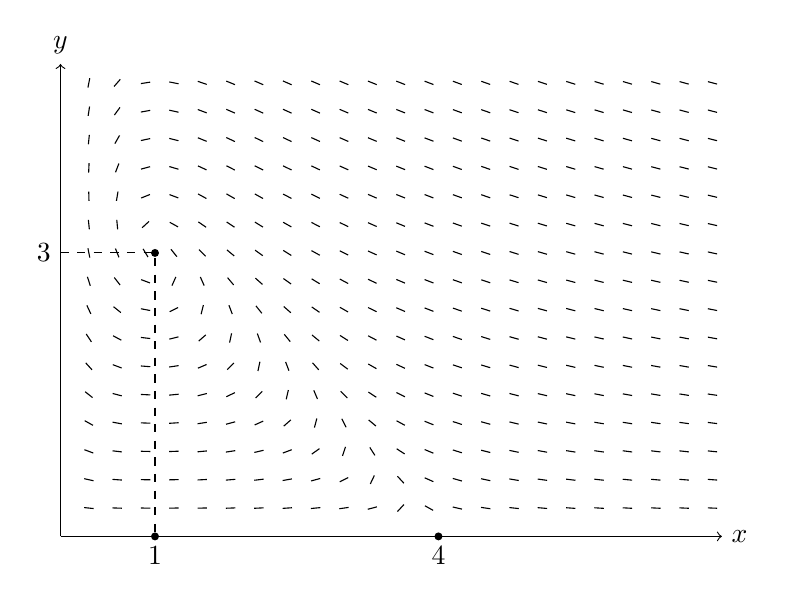
\begin{tikzpicture}[scale=1.2, /pgf/fpu/install only={reciprocal}]
    \draw[->] (0, 0) --  (0, 5) node[above] {$y$};
    \draw[->] (0, 0) --  (7, 0) node[right] {$x$};

    \draw[dashed] (0, 3) node[left] {3} -- (1, 3) -- (1, 0) node[below] {1};

    \fill (1, 3) circle (1.2pt);
    \fill (4, 0) circle (1.2pt) node[below] {4};
    \fill (1, 0) circle (1.2pt);

    \def\len{0.1}

    \foreach \x in {0.3, 0.6, ..., 7} {
        \foreach \y in {0.3, 0.6, ..., 5} {
            \pgfmathsetmacro{\m}{\y * (\x - 1)/(2 * \x * (4 - \x - \y))}
            \pgfmathsetmacro{\dx}{\len/sqrt(1+(\m)^2)}
            \pgfmathsetmacro{\dy}{\m*\dx}
            \draw (\x-\dx/2,\y-\dy/2)--(\x+\dx/2,\y+\dy/2);
        }
    }
  \end{tikzpicture}
  \end{center}
  Solutions flow in from the bottom left and right and spiral into the stable fixed point at $(1, 3)$.
\end{example}
\section{Partial Differential Equations}
\textit{Partial differential equations} (PDEs) are differential equations with multiple independent variables.

We are going to illustrate some introductory ideas with \textit{wave equations}.
\subsection{First Order Wave Equation}
Consider the function $\psi(x, t)$ where $x$ is position and $t$ is time governed by the PDE:
\[
  \pderiv{\psi}{t} - c \pderiv{\psi}{x} = 0
\]
where $c$ is a constant with dimensions of speed.

We can employ the \textit{method of characteristics} to solve this PDE.

How does $\psi$ vary along a path $x(t)$?
On the path we have $\psi(x(t), t)$ so we can use the multivariate chain rule (\cref{multivariateChainRule}) to yield:
\begin{align*}
  \pderiv{\psi}{t} &= \pderiv{\psi}{t} + \pderiv{\psi}{x} \deriv{x}{t} \\
                   &= \pderiv{\psi}{x}\left(c + \deriv{x}{t}\right)
\end{align*}
If we choose $x(t)$ such that $\deriv{x}{t} = -c$, then
\[
  x(t)  = x_0 - ct
\]
where $x_0$ is a constant on the path and is also used to label the path.

By construction, on such paths $\pderiv{\psi}{t} = 0$ so $\psi$ is constant along the path.
These paths are referred to as \textit{characteristics} of the PDE.
\begin{center}
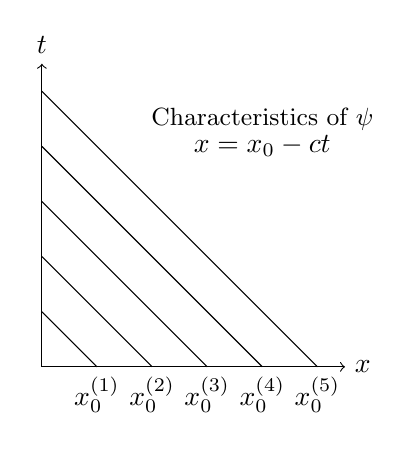
\begin{tikzpicture}[scale=0.7]
  \draw[->] (0, 0) --  (0, 5.5) node[above] {$t$};
  \draw[->] (0, 0) --  (5.5, 0) node[right] {$x$};

  \node at (4, 4) {$x = x_0 - ct$};
  \node at (4, 4.5) {\small Characteristics of $\psi$};

  \foreach \x in {1, 2, ..., 5} {
    \draw (0, \x) -- (\x, 0) node[below] {$x^{(\x)}_0$};
  }
\end{tikzpicture}
\end{center}
Since $\psi$ is constant along characteristics, suppose for each characteristic the value of $\psi$ is given by $f(x_0)$ for an arbitrary $f(x_0)$.
The general solution to the first order wave equation is then:
\[
  \psi(x, t) = f(x_0) = f(x + ct)
\]
for some arbitrary function $f$.
Differentiating this, we can easily check that every function of this form satisfies the PDE.
We also see that this satisfies the PDE with the initial condition $\psi(x, t=0) = f(x)$.
\end{document}
